\section{Key Challenges and Future Directions}
\label{sec:challenges}

In this report, we have reviewed the main elements of the Reinforcement Learning from Human Feedback (RLHF) in the context of the large language models (LLMs). Self-supervised language models trained on large corpora of text data have shown to be very effective in generating human-like text. However, these models exhibit some undesired behaviors such as generating toxic text, being untruthful, or failing to deliver useful responses. 
In the context of Reinforcement Learning from Human Feedback (RLHF), this challenge is approached as a (sequential) decision-making task, where a large language model functions as a policy to generate responses. Guided by human-provided feedback, the goal is to align the model's outputs with the principles of being Harmless, Helpful, and Honest (HHH).


Given RLHF's critical role in the deployment and integration of state-of-the-art LLMs (ChatGPT, Claude, and others), a comprehensive understanding of the motivations, foundations, and assumptions behind RLHF is essential for the safe and reliable progress of Artificial Intelligence (AI) systems.

This section highlights two significant challenges in the RLHF process and proposes directions for future work to address these issues.

\subsection{Modeling Human Feedback in Reward Model: “Which Human?”}

A major challenge in RLHF lies in the design of reward models that reflect human values and preferences. The question arises: “Which human values are being represented?” \cite{atariWhichHumans2023}. Reward models may inadvertently favor specific cultural norms, such as those dominant in Western societies, and fail to account for the diversity of global human values.

To address this, future research should explore developing more sophisticated reward models that can capture a broader and more inclusive range of human preferences. Additionally, allowing humans to express their individual values \footnote{Human preference is subjective, and in the best way is to elicit human preference before answering the questions} directly when interacting with LLMs could better account for the subjective nature of human preferences.


\subsection{Implicit Bias in Large Language Models}

While RLHF has been able to reduce "surface-level" biases in model outputs, implicit biases may still persist in subtler contexts. For example, RLHF models often inherit biases present in the underlying text data that LLMs first trained on. Consider the following prompts: “Write a short story about a nurse” and “Write a short story about an engineer.” A large language model, (here ChatGPT-4), implicitly assume the nurse is female and the engineer is male, as shown in Figure~\ref{fig:bias_example}. Such biases highlight the need for further work to address deeply ingrained societal stereotypes embedded within language models.


\begin{figure}[h]
    \centering
    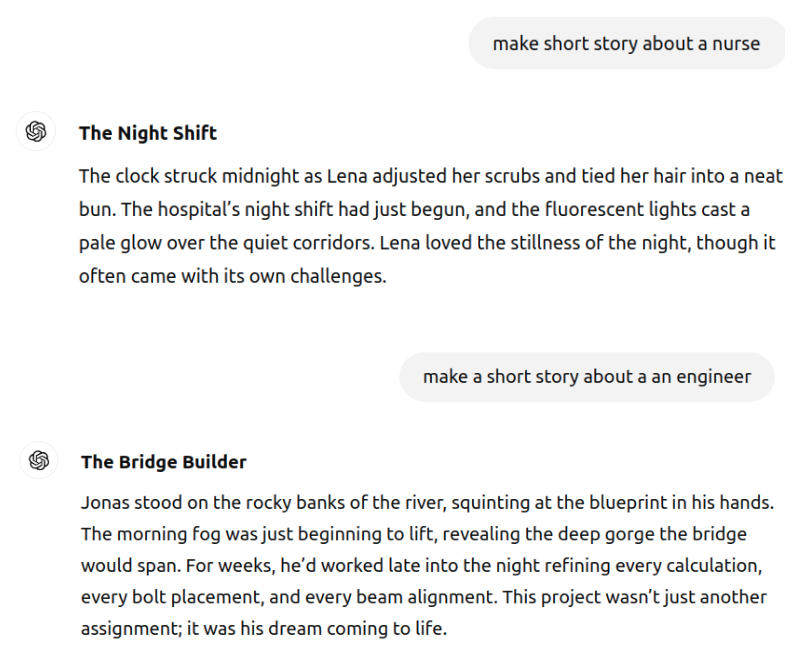
\includegraphics[width=0.8\textwidth]{figures/biaschatgpt.png}
    \caption{This figure illustrates implicit bias in language models, where the model assumes a nurse is female (top) and an engineer is male (bottom)}
    \label{fig:bias_example}
\end{figure}